
\documentclass[mathserif,11pt]{beamer}

\mode<presentation>
{
\usetheme{default}
}


\title[] % (optional, use only with long paper titles)
{An evolutionary model of plant succession}
% \subtitle
% {Include Only If Paper Has a Subtitle}

\author[Falster, Falster]
{
  Daniel~Falster\inst{1} \and
  \textcolor{green!50!black}{Daniel~Falster}\inst{2}
}

\institute[Macquarie University, latex land and others]
{
  \inst{1}%
  Macquarie University, Australia
  \and
  \vskip-2mm
  \inst{2}%
  latex land, Earth
}


% Includes for frame package
\usepackage{framed,color}
\definecolor{shadecolor}{rgb}{0.5,0.5,0.5}

% Make a custom block
\newenvironment<>{customBlock}[1]{%
  \begin{actionenv}#2%
      \def\insertblocktitle{#1}%
      \par%
      \mode<presentation>{%
        \setbeamercolor{block title}{fg=white,bg=orange!20!black}
       \setbeamercolor{block body}{fg=black,bg=olive!50}
       \setbeamercolor{itemize item}{fg=orange!20!black}
       \setbeamertemplate{itemize item}[triangle]
     }%
      \usebeamertemplate{block begin}}
    {\par\usebeamertemplate{block end}\end{actionenv}}


% Define new environments for mdframed package
\usepackage{tikz}
\usepackage[framemethod=tikz]{mdframed}

\newmdenv[outerlinewidth=3,leftmargin=0,%
rightmargin=20,backgroundcolor=white,%
outerlinecolor=black,innertopmargin=2pt,%
splittopskip=\topskip,skipbelow=\baselineskip,%
skipabove=\baselineskip]{titleBox}

\newmdenv[tikzsetting={draw=black,fill=white,fill opacity=0.7, line width=4pt},backgroundcolor=none,leftmargin=0,rightmargin=40,innertopmargin=4pt,skipbelow=\baselineskip,%
skipabove=\baselineskip]{transparentTitleBox}
%http://tex.stackexchange.com/questions/38281/transparent-background-for-mdframed-environment


%----------------------------------------------------------------------------------------
\begin{document}

{%title with image as background
  \usebackgroundtemplate{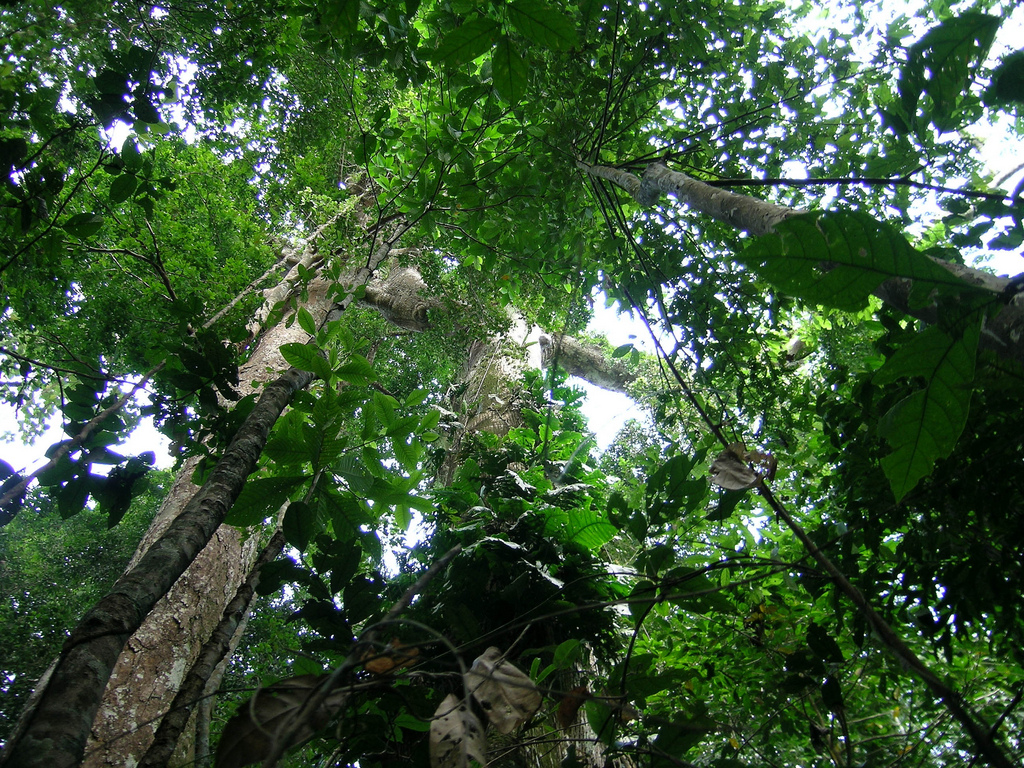
\includegraphics[width=1.0\paperwidth]{images/Background.jpg}}
  \begin{frame}[plain] 

  \begin{shaded}
  A block made with frame package
  \end{shaded}

  \begin{customBlock}{A customized  block}
    First.
  \end{customBlock}

  \begin{titleBox}
  A frame made with mdframed
  \end{titleBox}
   

  \begin{transparentTitleBox}
  {\huge transparent mdframed?}
  \end{transparentTitleBox}


  \end{frame}
}

{% Example using built-in title functions
  \usebackgroundtemplate{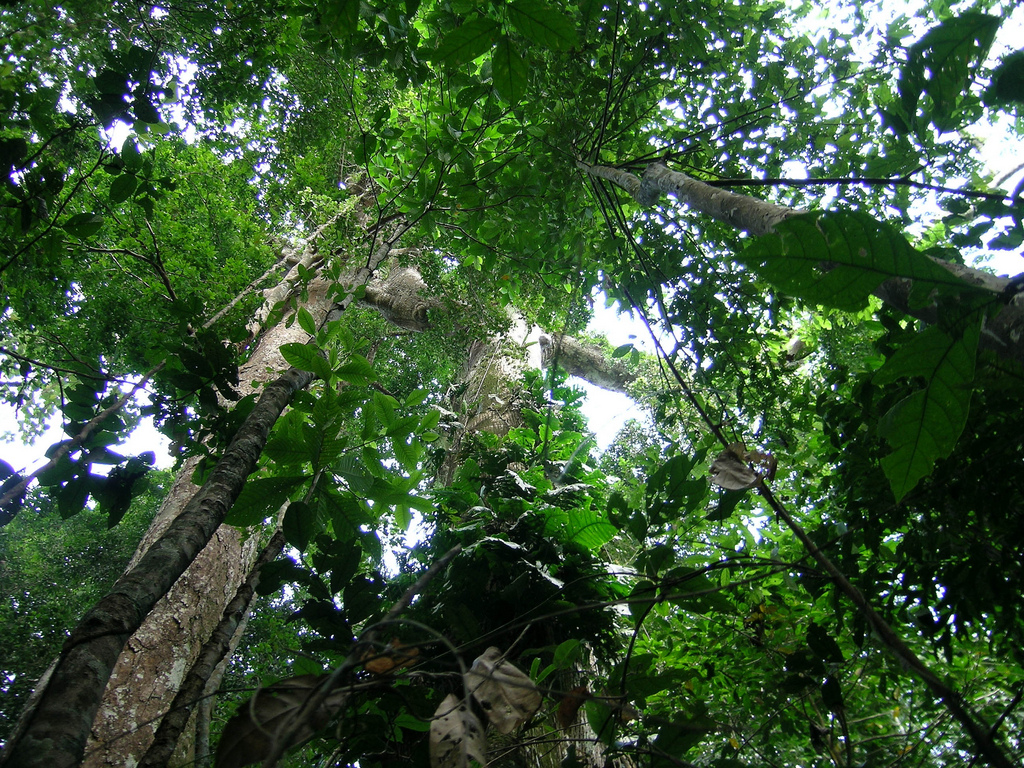
\includegraphics[width=1.0\paperwidth]{images/Background.jpg}}
  \begin{frame}[plain] 

  \begin{transparentTitleBox}
  \maketitle  
  \end{transparentTitleBox}

  \end{frame}
}

{%title with image as background
  \usebackgroundtemplate{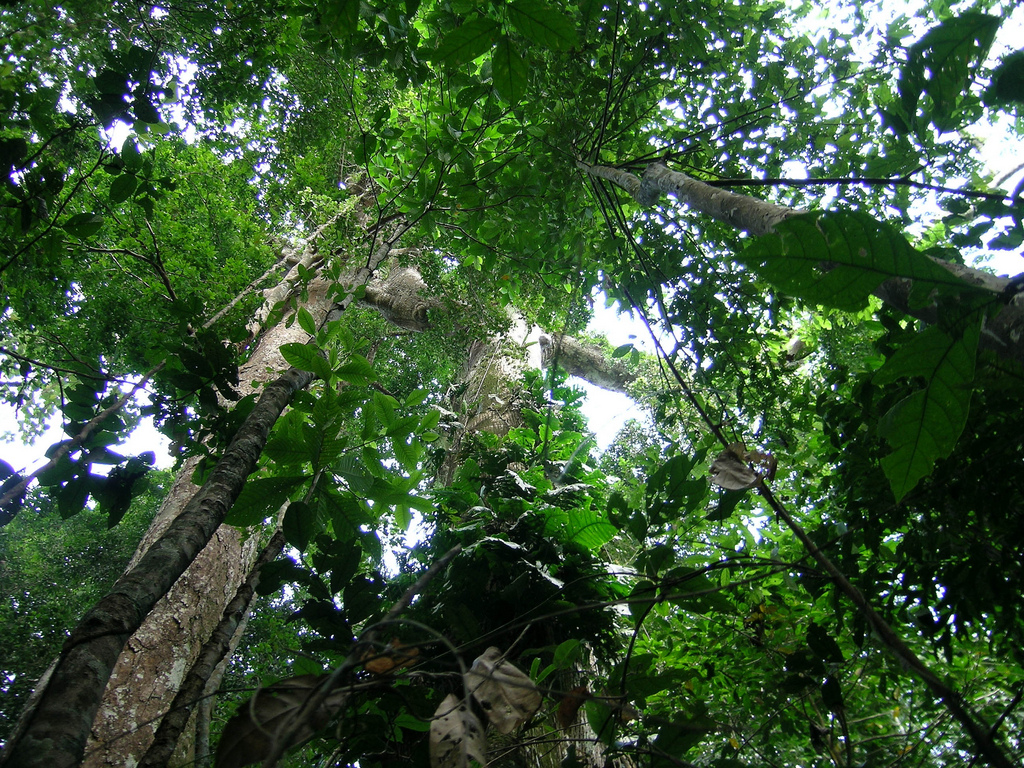
\includegraphics[width=1.0\paperwidth]{images/Background.jpg}}
  \begin{frame}[plain] 

  \begin{transparentTitleBox}
  {\huge \inserttitle}
  \end{transparentTitleBox}

   \begin{transparentTitleBox}
   {\tiny
    \insertauthor \\[\baselineskip]
%    \insertshortauthor \\[\baselineskip]
%    \insertshortinstitute
     \insertinstitute   
    }
   \end{transparentTitleBox}

  \end{frame}
}

%-----------------------------------
\end{document}